% Faithful native paths from source/普通高考/2009/2009新课标文(海南,宁夏).pdf, page 1.
% Original outlines, connected rock fissures, solid/dashed edges and shaded regions retained.
% Labels retain their original objects; no arbitrary geometric substitute or raster wrapper.
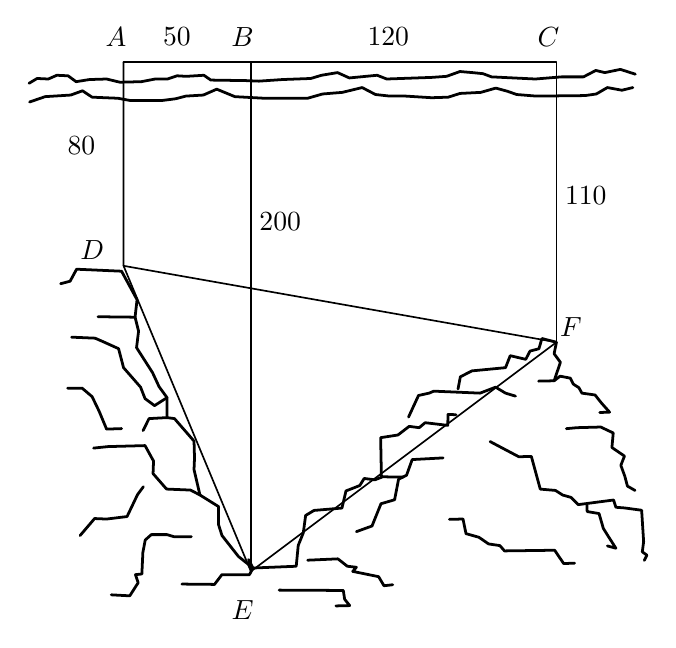
\begin{tikzpicture}[x=1cm,y=1cm,font=\normalsize,line join=round,line cap=round]
\path[draw=black,line width=1.0pt] (0.39810,7.29693) -- (0.49996,7.35805) -- (0.64251,7.35124) -- (0.75119,7.39879) -- (0.89374,7.39198) -- (0.99561,7.31730) -- (1.16534,7.34443) -- (1.38263,7.35124) -- (1.55237,7.31049) -- (1.82397,7.31730) -- (2.00051,7.35124) -- (2.15669,7.35124) -- (2.27886,7.39198) -- (2.39429,7.38517) -- (2.61839,7.39879) -- (2.70664,7.33767) -- (3.15478,7.33086) -- (3.31771,7.32411) -- (3.61649,7.34443) -- (3.97634,7.35805) -- (4.11214,7.39879) -- (4.31581,7.43273) -- (4.46523,7.36486) -- (4.81826,7.39879) -- (4.94050,7.35124) -- (5.51083,7.37161) -- (5.70093,7.38517) -- (5.87067,7.44629) -- (6.02690,7.43273) -- (6.16264,7.41911) -- (6.27132,7.37842) -- (6.82803,7.35124) -- (7.16080,7.37842) -- (7.43915,7.37842) -- (7.59533,7.45985) -- (7.71075,7.43273) -- (7.90767,7.47348) -- (8.09778,7.41235) ;
\path[draw=black,line width=1.0pt] (0.40488,7.05930) -- (0.60180,7.12717) -- (0.92771,7.14754) -- (1.07707,7.20185) -- (1.19930,7.12042) -- (1.52521,7.10680) -- (1.67458,7.07967) -- (2.09554,7.07967) -- (2.25852,7.10005) -- (2.38752,7.13398) -- (2.61156,7.14754) -- (2.78135,7.22222) -- (3.01215,7.12717) -- (3.38561,7.10680) -- (3.93556,7.10680) -- (4.12573,7.16111) -- (4.37696,7.18153) -- (4.62812,7.24260) -- (4.79792,7.15435) -- (4.98122,7.13398) -- (5.18495,7.13398) -- (5.51080,7.11361) -- (5.72133,7.12042) -- (5.87070,7.16792) -- (6.13549,7.18153) -- (6.32559,7.23579) -- (6.47502,7.19510) -- (6.59039,7.15435) -- (6.84162,7.13398) -- (7.45950,7.14079) -- (7.60211,7.16111) -- (7.74280,7.24271) -- (7.92801,7.20866) -- (8.06615,7.24271) ;
\path[draw=black,line width=1.0pt] (0.79877,4.75162) -- (0.91938,4.78334) -- (1.00186,4.93567) -- (1.57295,4.91029) -- (1.76969,4.54853) -- (1.74431,4.32646) ;
\path[draw=black,line width=1.0pt] (1.27473,4.33207) -- (1.74430,4.32648) -- (1.78871,4.14877) -- (1.76333,3.93934) -- (1.96642,3.62210) -- (2.04890,3.44439) -- (2.15041,3.30481) -- (2.15041,3.05096) ;
\path[draw=black,line width=1.0pt] (0.93837,4.07262) -- (1.23664,4.05993) -- (1.33815,4.01552) -- (1.53490,3.92669) -- (1.59811,3.68524) -- (1.81412,3.43804) -- (1.87122,3.29211) -- (1.99177,3.20322) -- (2.15045,3.30480) ;
\path[draw=black,line width=1.0pt] (0.88762,3.42536) -- (1.07162,3.42536) -- (1.19857,3.31749) -- (1.28740,3.13344) -- (1.38263,2.90497) -- (1.57297,2.91138) ;
\path[draw=black,line width=1.0pt] (1.84583,2.88597) -- (1.92150,3.03848) -- (2.15043,3.05099) -- (2.24490,3.03848) -- (2.49310,2.75273) -- (2.49945,2.53695) -- (2.49310,2.39096) -- (2.56836,2.06826) ;
\path[draw=black,line width=1.0pt] (1.21761,2.66386) -- (1.40160,2.68289) -- (1.87123,2.69558) -- (1.97909,2.49890) -- (1.97275,2.34022) -- (2.14405,2.14353) -- (2.44866,2.13079) -- (2.56833,2.06827) -- (2.80408,1.92141) -- (2.80408,1.69294) -- (2.84849,1.55336) -- (3.05786,1.28683) -- (3.24192,1.14090) -- (3.18482,1.24876) ;
\path[draw=black,line width=1.0pt] (1.04627,1.55334) -- (1.23027,1.76906) -- (1.38260,1.76278) -- (1.64273,1.79450) -- (1.77603,2.07373) -- (1.85001,2.17315) ;
\path[draw=black,line width=1.0pt] (1.44212,0.80035) -- (1.67699,0.78755) -- (1.78380,0.95414) -- (1.74958,1.05659) -- (1.83078,1.06514) -- (1.84358,1.33849) -- (1.87345,1.49647) -- (1.95033,1.56486) -- (2.15104,1.56486) -- (2.23649,1.53919) -- (2.45856,1.53919) ;
\path[draw=black,line width=1.0pt] (2.33898,0.93703) -- (2.75324,0.93278) -- (2.84719,1.05665) -- (3.19737,1.05665) -- (3.24190,1.14087) -- (3.79105,1.16340) -- (3.81665,1.42819) -- (3.88068,1.58617) -- (3.91060,1.80829) -- (4.01736,1.87232) -- (4.37184,1.90224) -- (4.42313,2.12005) -- (4.59822,2.18839) -- (4.65375,2.27809) -- (4.79042,2.26098) -- (4.88862,2.29940) -- (5.14916,2.29514) ;
\path[draw=black,line width=1.0pt] (3.57323,0.86017) -- (4.38896,0.85592) -- (4.40601,0.74486) -- (4.47010,0.66371) -- (4.29495,0.65947) ;
\path[draw=black,line width=1.0pt] (3.93625,1.24026) -- (4.32060,1.25731) -- (4.44015,1.16336) -- (4.55553,1.15056) -- (4.50872,1.09805) -- (4.83737,1.03100) -- (4.90571,0.91569) -- (5.01671,0.92849) ;
\path[draw=black,line width=1.0pt] (4.55533,1.60287) -- (4.75359,1.67458) -- (4.86745,1.95718) -- (5.04039,2.00776) -- (5.09103,2.26929) -- (5.19219,2.31988) -- (5.26390,2.51814) -- (5.65617,2.53921) ;
\path[draw=black,line width=1.0pt] (5.73631,1.75892) -- (5.90925,1.76317) -- (5.94720,1.57754) -- (6.11170,1.53115) -- (6.23400,1.44681) -- (6.37742,1.42568) -- (6.43644,1.35822) -- (7.07336,1.36666) -- (7.18722,1.19797) -- (7.32639,1.20216) ;
\path[draw=black,line width=1.0pt] (4.87291,2.29326) -- (4.86325,2.79647) -- (5.08258,2.83023) -- (5.22594,2.93989) -- (5.35249,2.92301) -- (5.42839,2.98629) -- (5.71524,2.95252) -- (5.71943,3.09170) -- (5.82066,3.08751) ;
\path[draw=black,line width=1.0pt] (5.21753,3.05799) -- (5.26811,3.16766) -- (5.34407,3.33216) -- (5.47894,3.36184) -- (5.53808,3.38699) -- (6.12575,3.36184) -- (6.32261,3.43757) -- (6.44916,3.36184) -- (6.57564,3.32372) ;
\path[draw=black,line width=1.0pt] (6.25283,2.74696) -- (6.61768,2.55405) -- (6.77706,2.55825) -- (6.89033,2.14299) -- (7.08323,2.12622) -- (7.17556,2.06749) -- (7.28038,2.03815) -- (7.37265,1.94589) -- (7.82143,2.00463) -- (7.85077,1.91231) -- (7.95985,1.90393) -- (8.17790,1.87459) -- (8.20310,1.47616) -- (8.18634,1.34612) -- (8.24501,1.30415) -- (8.21149,1.23709) ;
\path[draw=black,line width=1.0pt] (7.74278,1.42144) -- (7.85076,1.39228) -- (7.75431,1.54327) -- (7.69138,1.64392) -- (7.63690,1.83263) -- (7.48591,1.85777) -- (7.48259,1.96028) ;
\path[draw=black,line width=1.0pt] (8.09403,2.12622) -- (7.99758,2.18076) -- (7.96405,2.30660) -- (7.91370,2.44497) -- (7.95980,2.56243) -- (7.80043,2.67145) -- (7.81719,2.85597) -- (7.65787,2.93147) -- (7.35589,2.92309) -- (7.22166,2.91052) ;
\path[draw=black,line width=1.0pt] (7.64527,3.11603) -- (7.77111,3.12022) -- (7.66622,3.23768) -- (7.58653,3.33832) -- (7.41936,3.36184) -- (7.38106,3.43058) -- (7.30975,3.47674) -- (7.27198,3.55224) -- (7.14200,3.57739) -- (7.06650,3.51865) -- (6.86935,3.51446) ;
\path[draw=black,line width=1.0pt] (5.84599,3.41381) -- (5.87533,3.56900) -- (6.02213,3.64449) -- (6.44915,3.68530) -- (6.50869,3.83745) -- (6.70578,3.79129) -- (6.76032,3.89613) -- (6.87354,3.92552) -- (6.91132,4.05550) -- (7.09595,4.00864) -- (7.06650,3.86260) -- (7.14619,3.75352) -- (7.06650,3.51871) ;
\path[draw=black,line width=0.6pt] (1.59814,7.56602) -- (7.09592,7.56602) -- (7.09592,4.00862) ;
\path[draw=black,line width=0.6pt] (3.21514,1.09804) -- (7.09589,4.00863) ;
\path[draw=black,line width=0.6pt] (3.21514,1.09804) -- (1.59816,4.97879) -- (1.59816,7.56604) ;
\path[draw=black,line width=0.6pt] (1.59814,4.97882) -- (7.09592,4.00866) ;
\path[draw=black,line width=0.6pt] (3.21514,7.56602) -- (3.21514,1.09803) ;
\node[anchor=base west,inner sep=0pt,outer sep=0pt] at (1.36894,7.76313) {$A$};
\node[anchor=base west,inner sep=0pt,outer sep=0pt] at (2.96798,7.76313) {$B$};
\node[anchor=base west,inner sep=0pt,outer sep=0pt] at (3.32439,5.42868) {$200$};
\node[anchor=base west,inner sep=0pt,outer sep=0pt] at (2.10103,7.77500) {$50$};
\node[anchor=base west,inner sep=0pt,outer sep=0pt] at (6.85566,7.76313) {$C$};
\node[anchor=base west,inner sep=0pt,outer sep=0pt] at (4.69712,7.77500) {$120$};
\node[anchor=base west,inner sep=0pt,outer sep=0pt] at (1.04961,5.05702) {$D$};
\node[anchor=base west,inner sep=0pt,outer sep=0pt] at (0.88663,6.39890) {$80$};
\node[anchor=base west,inner sep=0pt,outer sep=0pt] at (2.97194,0.48330) {$E$};
\node[anchor=base west,inner sep=0pt,outer sep=0pt] at (7.14396,4.08687) {$F$};
\node[anchor=base west,inner sep=0pt,outer sep=0pt] at (7.20514,5.75209) {$110$};
\end{tikzpicture}
